\documentclass[a4paper]{article}
% standard packages
\usepackage{amssymb}
\usepackage{euscript}
\usepackage{eurosym}
\usepackage{graphicx}
\graphicspath{{img/}}
\usepackage{color}
\usepackage{epsfig}
\usepackage{fullpage}
\usepackage[colorlinks=true]{hyperref}
\usepackage{titling}

% title style
\pretitle{\noindent\LARGE}
\posttitle{\\[1ex]}
\preauthor{\large}
\postauthor{,}
\predate{\large(}
\postdate{)}
\date{last update: \today}

% large page size
\oddsidemargin -1cm
\topmargin -1cm
\textwidth 18cm
\textheight 27cm
\pagestyle{empty}


% PDF figure (floating)
\newcommand{\image}[3]{
\begin{figure}[#1]
\begin{center}
\caption{\small#3}
\includegraphics{img_#2.pdf}
\label{image:#2}
\end{center}
\end{figure}
}

% simple image
\newcommand\simpleimage[3][\linewidth]{
\smallskip\begin{center}\vbox{\noindent
\includegraphics[width=#1]{#2}\\%
\parbox{#1}{\it#3}}\end{center}
\medskip}

%\newcommand\simpleimage[3][\linewidth]{
%\smallskip\vbox{\noindent
%\includegraphics[width=#1]{#2}\\%
%\it#3}
%\medskip}


% companies
\def\SchaefferAG{\href{https://www.schaeffer-ag.de/en/}{Schaeffer-AG}}
\def\MultiCB{\href{https://portal.multi-circuit-boards.eu}{Multi-CB}}
\def\BlueFors{\href{https://www.bluefors.com/}{BlueFors}}

\def\Ohmite{\href{https://www.ohmite.com}{Ohmite}}
\def\Firmetal{\href{http://www.firmetal.com}{Firmetal}}
\def\Bruker{\href{https://www.bruker.com}{Brucker}}

% use this to refer to Farnell and RS numbers:
\def\FarnellN#1{\href{https://fi.farnell.com/#1}{Farnell:#1}}
\def\RSN#1{\href{https://fi.rsdelivers.com/productlist/search?query=#1}{RS:#1}}

% products:
\def\OhmiteOFOD{\href{https://www.ohmite.com/assets/docs/res_od_of_oa.pdf}{Ohmite OF/OD series}}

% Supplementary materials on github <report> <file>
\def\GitFile#1#2{\href{https://github.com/slazav/he3notes/raw/master/#1/#2}{#1/#2}}

% Supplementary materials on my users.aalt.fi page
\def\WWWFile#1{\href{https://users.aalto.fi/~zavyalv1/#1}{#1}}


%progams
\def\MagnettiProg{\href{https://github.com/slazav/magneetti}{\tt magnetti}}



\title{Carbon thermometers for dilution fridges}
\author{V.Zavjalov}

\twocolumn
\begin{document}
\maketitle

The goal is to make standard thermometers for use in dilution fridges. I
use carbon \Ohmite{} resistors (\OhmiteOFOD{}, \FarnellN{2427380},
\FarnellN{2427405}, \RSN{892-5449} etc.), which are claimed to be
good thermometers at millikelvin temperatures~\cite{therm_paper}. The
series OD and OF have different sizes (diameter $2.5$~mm and~$3.8$~mm and
length~$7$~mm and~$10$~mm respectively). I grind resistors down to
approximately $0.7$~mm thickness and glue it in a slit in a copper box
using Stycast 2850. This provides a good thermal contact with the box,
mechanical stability, and protection against moisture.

\begin{center}
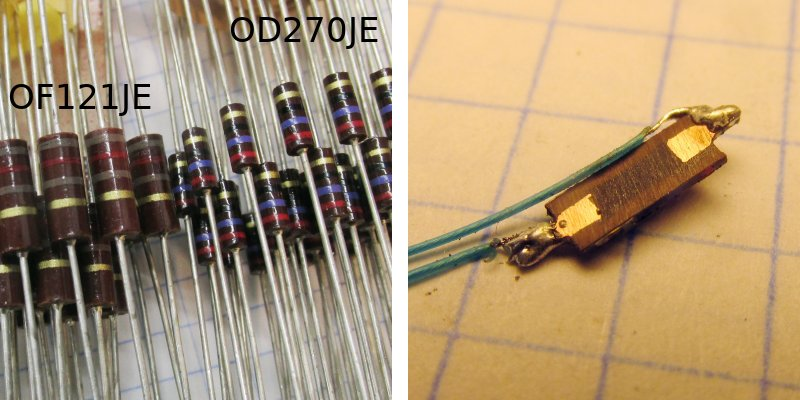
\includegraphics[width=\linewidth]{img/res.jpg}
\end{center}

Copper boxes are ordered in \SchaefferAG.  The
box has $30\times30\times5$~mm size. It contains a~$20\times18\times3$~mm
compartment for RC lowpass filters, a $1\times16\times4$~mm slit for the
resistor and a~$16\times7\times3$~mm additional compartment which can be
used for sample chips. Holes are compatable with standard~$20\times20$ M4
hole grid on \BlueFors{} refrigerator plates. Drawings in FPD format are
available~\cite{box_drawings}, price was 315\euro{} for 10 boxes and 10
lids.

\begin{center}
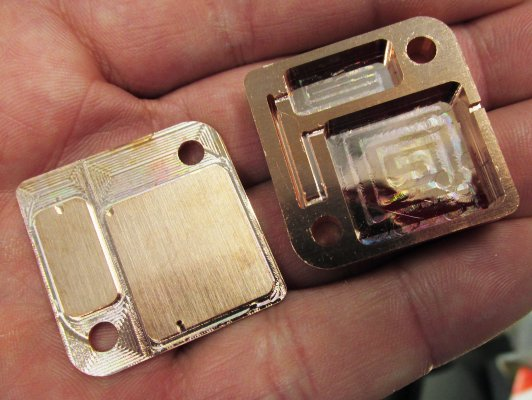
\includegraphics[width=\linewidth]{img/box.jpg}
\end{center}

PCBs for filters are ordered in \MultiCB. Price
is 75\euro{} for 10 boards with two different filters and two small
sample plates each. Kicad project~\cite{filterpcb-kicad} and Gerber
files~\cite{filterpcb-gerber} are available.

To connect thermometers to BlueFors 4-pin sockets we use inserts
of LEMO {\tt FFA.0S.304.CLAC44} connectors (\FarnellN{2442870}).

\begin{center}
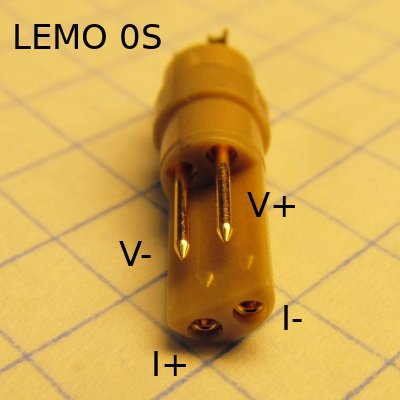
\includegraphics[width=3.5cm]{img/conn.jpg}
\end{center}

\subsection*{List of devices}

\noindent
\begin{tabular}{|ll lll l|}\hline
N& Resistor& $R_0$ & $R_1$ & $R_2$ & \\
\hline
2018-11-02 N1&OD270JE& 27  & 56  & 56.0&\\
2018-11-02 N2&OD270JE& 27  & 59  & 64.4&\\
2018-11-02 N3&OF121JE& 120 & 231 & 277&\\
\hline
\end{tabular}
\medskip

Here $R_0$, $R_1$, and $R_2$ are nominal resistance, resistance after
grinding, and resistance after soldering and glueing. Change during
glueing probably means that contacts with carbon in the resistor
after grinding are not stable.

{\bf Work in progress...}

\begin{thebibliography}{}
\bibitem{therm_paper}
N. Samkharadze, A. Kumar, G. A. Cs{\'a}thy,
A New Type of Carbon Resistance Thermometer with.Excellent Thermal Contact at Millikelvin Temperatures,
{\it JLTP}, {\bf 160}, 246--253 (2010),\\
\url{https://doi.org/10.1007/s10909-010-0192-5}

\bibitem{box_drawings}
Box drawing in FrontPanel Disigner format, for production,\\
\WWWFile{notes/2018-thermbox/box\_v1.zip}

\bibitem{filterpcb-kicad}
Filter PCB, KiCAD project,\\
\WWWFile{notes/2018-thermbox/pcb\_kicad.zip}

\bibitem{filterpcb-gerber}
Filter PCB, Gerber files for production,\\
\WWWFile{notes/2018-thermbox/pcb\_v1.zip}

\end{thebibliography}
\end{document}
